%
% File udst2018.tex

\documentclass[11pt,a4paper]{article}
\usepackage[hyperref]{udst2018}
\usepackage{times}
\usepackage{latexsym}
\usepackage{amsmath}
\usepackage{tikz}
\usepackage{tikz-dependency}
\usepackage[warn]{textcomp}
\usepackage[font=small]{caption}
\usepackage{subcaption}
\usepackage{multirow}
\usepackage{url}
\usepackage{etoolbox}
\usepackage{xr}
\usepackage{adjustbox}

\newcommand{\com}[1]{}
\newcommand{\oa}[1]{\footnote{\color{red}OA: #1}}
\newcommand{\daniel}[1]{\footnote{\color{blue}Daniel: #1}}


\hyphenation{SemEval}

\DeclareMathOperator*{\argmin}{argmin}
\DeclareMathOperator*{\argmax}{argmax}

\makeatletter
\patchcmd\@combinedblfloats{\box\@outputbox}{\unvbox\@outputbox}{}{%
   \errmessage{\noexpand\@combinedblfloats could not be patched}%
}%
 \makeatother


\usetikzlibrary{shapes,shapes.misc}


\aclfinalcopy 
\def\aclpaperid{***} %  Enter the Paper ID here for final camera ready copy

%\setlength\titlebox{5cm}
% You can expand the titlebox if you need extra space
% to show all the authors. Please do not make the titlebox
% smaller than 5cm (the original size); we will check this
% in the camera-ready version and ask you to change it back.

\title{HUJI at the CoNLL 2018 UD Shared Task: \\
Universal Dependency Parsing with a Transition-Based DAG Parser}

\author{Daniel Hershcovich$^{1,2}$ \\
  \\\And
  Omri Abend$^2$ \\
  $^1$The Edmond and Lily Safra Center for Brain Sciences \\
  $^2$School of Computer Science and Engineering \\
  Hebrew University of Jerusalem \\
  \texttt{\{danielh,oabend,arir\}@cs.huji.ac.il}
  \\\And
  Ari Rappoport$^2$
}

\date{}

\begin{document}
\maketitle
\begin{abstract}
  We present TUPA, a neural transition-based general DAG parser,
  submitted by HUJI to the CoNLL 2018 UD shared task.
  TUPA was designed for parsing UCCA, a cross-linguistic
  semantic annotation scheme, exhibiting
  reentrancy, discontinuity and non-terminal nodes.
  By employing a conversion protocol to represent
  UD trees and graphs in a UCCA-like unified DAG format,
  we train TUPA without modification on the UD parsing task.
  Our code is available at \url{https://github.com/danielhers/tupa}.
\end{abstract}

\section{Introduction}\label{sec:introduction}

In this paper we describe the HUJI submission to the CoNLL 2018 shared task
on Universal Dependency parsing \cite{nivre2016universal,11234/1-2515}.
We focus only on parsing, using a baseline model \cite[UDPipe;][]{udpipe:2017}
for tokenization, sentence splitting, part-of-speech tagging and morphological tagging.
Our system is based on TUPA \cite{hershcovich2017a,hershcovich2018multitask},
a transition-based UCCA parser.
UCCA \cite[Universal Conceptual Cognitive Annotation;][]{abend2013universal} is a
cross-linguistic semantic annotation scheme, representing scenes, participants,
attributes and relations in a directed acyclic graph (DAG) structure,
and allowing reentrancy (argument sharing),
discontinuity (corresponding to non-projectivity in dependency annotations)
and non-terminal nodes (as opposed to dependencies, which are bi-lexical).
To parse UD using TUPA, we employ a conversion protocol to represent
UD trees and graphs in a UCCA-like unified DAG format (\S\ref{sec:format}).

\begin{figure}[ht]
\begin{subfigure}{0.47\textwidth}
  \centering
    \begin{dependency}[text only label, label style={above}, font=\small]
    \begin{deptext}[column sep=.8em,ampersand replacement=\^]
    After \^ graduation \^ , \^ John \^ moved \^ to \^ Paris \\
    \end{deptext}
        \depedge{2}{1}{case}
        \depedge{4}{3}{punct}
        \depedge{5}{4}{nsubj}
        \depedge[edge end x offset=-2pt]{2}{5}{obl}
        \depedge{7}{6}{case}
        \deproot[edge unit distance=3ex]{5}{root}
        \depedge[edge unit distance=3ex]{5}{7}{obl}
    \end{dependency}
  \caption{\label{fig:original_examples}Example UD tree.}
\end{subfigure}
\begin{subfigure}{0.47\textwidth}
  \centering
  \scalebox{.95}{
  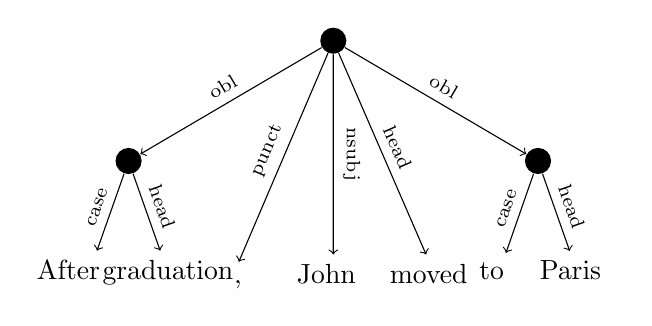
\begin{tikzpicture}[level distance=17mm, ->,
      every node/.append style={sloped,anchor=south,auto=false,font=\scriptsize},
      level 1/.style={sibling distance=13mm},
      level 2/.style={sibling distance=1cm}]
    \tikzstyle{word} = [font=\rmfamily,color=black]
    \node (ROOT) [fill=black,circle] {}
      child {node (after) [fill=black,circle] {}
      {
        child {node [word] {After{\color{white}g}\quad\quad} edge from parent node {case}}
        child {node [word] {\quad graduation\quad\quad} edge from parent node {head}}
      } edge from parent node {obl}}
      child {node {}
      {
        child {node [word] (comma) {\quad,{\color{white}g}} edge from parent [draw=none]}
      } edge from parent [draw=none]}
      child {node {}
      {
        child {node [word] (John) {John{\color{white}g}} edge from parent [draw=none]}
      } edge from parent [draw=none]}
      child {node {}
      {
        child {node [word] (moved) {moved{\color{white}g}} edge from parent [draw=none]}
      } edge from parent [draw=none]}
      child {node (to) [fill=black,circle] {}
      {
          child {node [word] {to{\color{white}g}} edge from parent node {case}}
          child {node [word] {Paris{\color{white}g}} edge from parent node {head}}
      } edge from parent node {obl}}
      ;
      \draw (ROOT) to node {punct} (comma);
      \draw (ROOT) to node {nsubj} (John);
      \draw (ROOT) to node {head} (moved);
  \end{tikzpicture}}
  \captionof{figure}{UD tree after conversion to unified DAG format.}\label{fig:converted_example_ud}
\end{subfigure}

\caption{UD tree before and after conversion to the unified DAG format.
Intermediate non-terminals and \textit{head} edges are introduced,
to get a constituency-like format.}\label{fig:converted_examples}
\end{figure}


%%%%%%%%%%%%%%%%%%%%%%%%%%%%%%%%%%%%%%%%%%%%%%%%%%%%%%%%%%%%%%%%%%%%%%%%%%%%%%%%%%%%%%%%
\section{Unified DAG Format}\label{sec:format}

To apply TUPA to UD parsing,
we convert it into a unified DAG format \cite{hershcovich2018multitask}.
The format consists of a rooted DAG, where the tokens are the terminal
nodes.\footnote{Our conversion code supports full conversion between UCCA and UD,
among other representation schemes,
and is publicly available at \url{http://github.com/danielhers/semstr/tree/master/semstr/conversion}.}
As in the UCCA format, edges are labeled (but not nodes),
and are divided into \textit{primary} and \textit{remote} edges,
where the primary edges form a tree (all nodes have at most one primary parent,
and the root has none).
Remote edges enable reentrancy, and thus together with primary edges
form a DAG.
Figure~\ref{fig:converted_examples} shows an example for a converted tree.

To convert UD into the unified DAG format,
we add a pre-terminal for each token,
and attach the pre-terminals according to the original dependency edges:
traversing the tree from the root down, for each head token we create a non-terminal
parent with the edge label {\it head},
and add the node's dependents as children of the created non-terminal node
(see Figure~\ref{fig:converted_example_ud}).

Any \textit{enhanced UD} heads beyond the normal head of a node are converted
to remote edges in the unified DAG format.



%%%%%%%%%%%%%%%%%%%%%%%%%%%%%%%%%%%%%%%%%%%%%%%%%%%%%%%%%%%%%%%
\section{General Transition-based DAG Parser}\label{sec:model}

We now turn to presenting TUPA \cite{hershcovich2017a,hershcovich2018multitask},
a general transition-based parser \cite{Nivre03anefficient}.
TUPA uses an extended set of transitions and features that supports
reentrancies, discontinuities and non-terminal nodes.
The parser state is composed of a buffer $B$ of tokens and nodes to be processed,
a stack $S$ of nodes currently being processed,
and a graph $G=(V,E,\ell)$ of constructed nodes and edges,
where $V$ is the set of \emph{nodes}, $E$ is the set of \emph{edges},
and $\ell : E \to L$ is the \emph{label} function, $L$ being the set of possible labels.
Some states are marked as \textit{terminal}, meaning that $G$ is the final output.
A classifier is used at each step to select the next transition based on features
encoding the parser's current state.
During training, an oracle creates training instances for the classifier,
based on gold-standard annotations.

\begin{figure*}
	\begin{adjustbox}{width=\textwidth,margin=3pt,frame}
	\begin{tabular}{llll|l|llllc|c}
		\multicolumn{4}{c|}{\textbf{\small Before Transition}} & \textbf{\small Transition} & \multicolumn{5}{c|}{\textbf{\small After Transition}} & \textbf{\small Condition} \\
		\textbf{\footnotesize Stack} & \textbf{\footnotesize Buffer} & \textbf{\footnotesize Nodes} & \textbf{\footnotesize Edges} & & \textbf{\footnotesize Stack} & \textbf{\footnotesize Buffer} & \textbf{\footnotesize Nodes} & \textbf{\footnotesize Edges} & \textbf{\footnotesize Terminal?} & \\
		$S$ & $x \;|\; B$ & $V$ & $E$ & \textsc{Shift} & $S \;|\; x$ & $B$ & $V$ & $E$ & $-$ & \\
		$S \;|\; x$ & $B$ & $V$ & $E$ & \textsc{Reduce} & $S$ & $B$ & $V$ & $E$ & $-$ & \\
		$S \;|\; x$ & $B$ & $V$ & $E$ & \textsc{Node$_X$} & $S \;|\; x$ & $y \;|\; B$ & $V \cup \{ y \}$ & $E \cup \{ (y,x)_X \}$ & $-$ &
		$x \neq \mathrm{root}$ \\
		$S \;|\; y,x$ & $B$ & $V$ & $E$ & \textsc{Left-Edge$_X$} & $S \;|\; y,x$ & $B$ & $V$ & $E \cup \{ (x,y)_X \}$ & $-$ &
		\multirow{4}{50pt}{\vspace{-5mm}\[\left\{\begin{array}{l}
		x \not\in w_{1:n},\\
		y \neq \mathrm{root},\\
		y \not\leadsto_G x
		\end{array}\right.\]} \\
		$S \;|\; x,y$ & $B$ & $V$ & $E$ & \textsc{Right-Edge$_X$} & $S \;|\; x,y$ & $B$ & $V$ & $E \cup \{ (x,y)_X \}$ & $-$ & \\
		$S \;|\; y,x$ & $B$ & $V$ & $E$ & \textsc{Left-Remote$_X$} & $S \;|\; y,x$ & $B$ & $V$ & $E \cup \{ (x,y)_X^* \}$ & $-$ & \\
		$S \;|\; x,y$ & $B$ & $V$ & $E$ & \textsc{Right-Remote$_X$} & $S \;|\; x,y$ & $B$ & $V$ & $E \cup \{ (x,y)_X^* \}$ & $-$ & \\
		$S \;|\; x,y$ & $B$ & $V$ & $E$ & \textsc{Swap} & $S \;|\; y$ & $x \;|\; B$ & $V$ & $E$ & $-$ &
		$\mathrm{i}(x) < \mathrm{i}(y)$ \\
		$[\mathrm{root}]$ & $\emptyset$ & $V$ & $E$ & \textsc{Finish} & $\emptyset$ & $\emptyset$ & $V$ & $E$ & $+$ & \\
	\end{tabular}
	\end{adjustbox}
	\caption{\label{fig:transitions}
	  The transition set of TUPA.
	  We write the stack with its top to the right and the buffer with its head to the left.
	  $(\cdot,\cdot)_X$ denotes a primary $X$-labeled edge, and $(\cdot,\cdot)_X^*$ a remote $X$-labeled edge.
	  $\mathrm{i}(x)$ is a running index for the created nodes.
	  In addition to the specified conditions,
	  the prospective child in an \textsc{Edge} transition must not already have a primary parent.
	}
\end{figure*}

\paragraph{Transition Set.}
Given a sequence of tokens $w_1, \ldots, w_n$, we predict a UCCA graph $G$ over the sequence.
Parsing starts with a single node on the stack (an artificial root node), and the input tokens
in the buffer. Figure~\ref{fig:transitions} shows the transition set.


Given a sequence of tokens $w_1, \ldots, w_n$,
we predict a rooted graph $G$ whose terminals are the tokens.
Parsing starts with the root node on the stack,
and the input tokens in the buffer.

The TUPA transition set includes
the standard \textsc{Shift} and \textsc{Reduce} operations,
\textsc{Node$_X$} for creating a new non-terminal node and an $X$-labeled edge,
\textsc{Left-Edge$_X$} and \textsc{Right-Edge$_X$} to create a new primary $X$-labeled edge,
\textsc{Left-Remote$_X$} and \textsc{Right-Remote$_X$} to create a new remote $X$-labeled edge,
\textsc{Swap} to handle discontinuous nodes,
and \textsc{Finish} to mark the state as terminal.



\begin{figure}[t]
   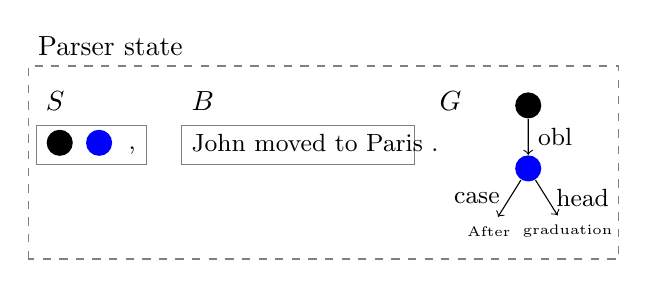
\begin{tikzpicture}[level distance=8mm, sibling distance=1cm]
   \node[anchor=west] at (0,1.5) {Parser state};
   \draw[color=gray,dashed] (0,-1.2) rectangle (7.5,1.25);
   \draw[color=gray] (.1,0) rectangle (1.5,.5);
   \node[anchor=west] at (.1,.8) {$S$};
   \node[fill=black, circle] at (.4,.275) {};
   \node[fill=blue, circle] at (.9,.275) {};
   \node[anchor=west] at (1.15,.175) {\small ,};
   \draw[color=gray] (1.95,0) rectangle (4.9,.5);
   \node[anchor=west] at (1.95,.8) {$B$};
   \node[anchor=west] at (1.95,.275) {\small John moved to Paris .};
   \node[anchor=west] at (5.1,.8) {$G$};
   \node[fill=black, circle] at (6.35,.75) {}
     child {node [fill=blue, circle] {}
     {
       child {node  {\tiny After} edge from parent [->] node[left] {\small case}}
       child {node {\tiny graduation} edge from parent [->] node[right] {\small head}}
     } edge from parent [->] node[right] {\small obl} };
   \end{tikzpicture}
   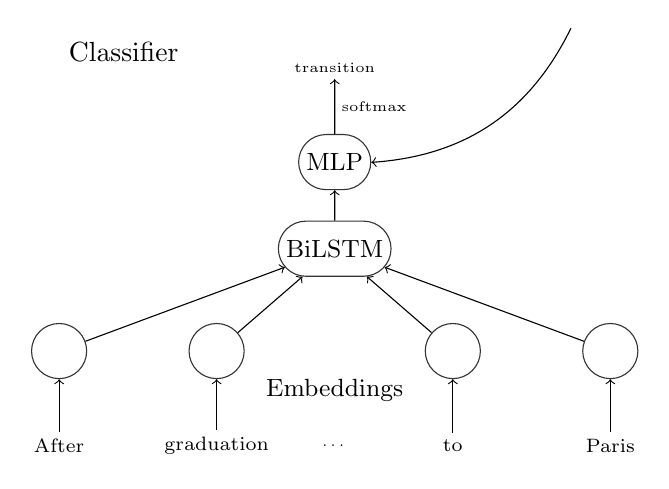
\begin{tikzpicture}[->]
   \node[anchor=west] at (0,6) {Classifier};
   \tiny
   \tikzstyle{main}=[rounded rectangle, minimum size=7mm, draw=black!80, node distance=12mm]
   \node[main] (specific) at (3.5,3.5) {\small BiLSTM};
   \node (embeddings) at (3.5,1.7) {\small Embeddings};
   \foreach \i/\word in {0/{After},2/{graduation},5/{to},7/{Paris}} {
       \node (x\i) at (\i,1) {\scriptsize \word};
       \node[main] (e\i) at (\i,2.2) {};
       \path (x\i) edge (e\i);
       \path (e\i) edge (specific);
   }
    \node (x4) at (3.5,1) {\ldots};
    \node[main] (mlp) at (3.5,4.6) {\small MLP};
    \path (specific) edge (mlp);
    \coordinate (state) at (6.5,6.3);
    \path (state) edge [bend left] (mlp);
    \node (transition) at (3.5,5.8) {transition};
    \path (mlp) edge node[right] {softmax} (transition);
   \end{tikzpicture}
\caption{Illustration of the TUPA model, from \citet{hershcovich2018multitask}.
Top: parser state (stack, buffer and intermediate graph).
		Bottom: BiLTSM architecture.
		Vector representation for the input tokens is computed
		by two layers of bidirectional LSTMs.
		The vectors for specific tokens are concatenated with
		embedding and numeric features from the parser state
		(for existing edge labels, number of children, etc.),
		and fed into the MLP for selecting the next transition.}\label{fig:single_model}
\end{figure}


%%%%%%%%%%%%%%%%%%%%%%%%%%%%%%%%%%%%%%%%%%%%%%%%%%%%%%%%%%%%%%%%%%%%%%%%%%%%%%%%%
\subsection{Transition Classifier}\label{sec:classifier}

To predict the next transition at each step,
we use a BiLSTM with embeddings as inputs,
followed by an MLP and a softmax layer for classification \cite{kiperwasser2016simple}.
The model is illustrated in Figure~\ref{fig:single_model}.
Inference is performed greedily,
and training is done with an oracle that yields the set of all optimal 
transitions at a given state (those that lead to a state from which the gold graph is still reachable).
Out of this set, the actual transition performed in training is the one
with the highest score given by the classifier,
which is trained to maximize the sum of log-likelihoods of all 
optimal transitions at each step.




\paragraph{Features.}

As features, we use vector embeddings
representing the words, lemmas, coarse POS tags, fine-grained POS tags,
punctuation, gap type, one-character prefix, three-character suffix,
shape (capturing orthographic features, e.g., ``Xxxx''), named entity type
(provided by spaCy \cite{spacy2}).\footnote{\url{http://spacy.io}}
and previously predicted edge labels and parser actions.
These embeddings are initialized randomly, except for the word embeddings,
which are initialized with the 250K most frequent word vectors from fastText
for each language
\cite{bojanowski2016enriching},\footnote{\url{http://fasttext.cc}}
pre-trained over Wikipedia and updated during training.

In addition to dropout between NN layers, we apply word dropout 
\cite{kiperwasser2016simple}: with a certain probability, the embedding for a
word is replaced with a zero vector. We do not apply word dropout to the external
word embeddings.

Finally, for all classifiers we add a novel real-valued feature to the input vector,
\textbf{ratio}, corresponding to the ratio between the number of terminals to number of nodes
in the graph $G$.
This feature serves as a regularizer for the creation of new nodes,
and should be beneficial for other transition-based constituency parsers too.


In addition, for each token
we use embeddings representing the 
To the learned word vectors, we concatenate 

Table~\ref{tab:features} lists all feature used for the classifier.
Numeric features are taken as they are, whereas categorical features are mapped to real-valued embedding
vectors.
For \texttt{w} features,
we concatenate randomly-initialized and pre-trained word embeddings.
For each node, we select a \textit{head terminal} by traversing the graph according to
a priority order on edge labels, taken from \citet{hershcovich2017a}.


\begin{table*}[h]
\centering
\begin{tabular}{l|l}
\bf Nodes & \bf Features \\ 
\hline
$s_0$ & \texttt{wmtuepT\#\^{}\$xhqyPCIEMN} \\
$s_1$ & \texttt{wmtueT\#\^{}\$xhyN} \\
$s_2$ & \texttt{wmtueT\#\^{}\$xhy} \\
$s_3$ & \texttt{wmtueT\#\^{}\$xhyN} \\
$b_0$ & \texttt{wmtuT\#\^{}\$hPCIEMN} \\
$b_1, b_2, b_3$ & \texttt{wmtuT\#\^{}\$} \\
$s_0l, s_0r, s_1l, s_1r, s_0ll, s_0lr, s_0rl, s_0rr, s_1ll, s_1lr, s_1rl, s_1rr$ &
    \texttt{wme\#\^{}\$} \\
$s_0L, s_0R, s_1L, s_1R, b_0L, b_0R$ & \texttt{wme\#\^{}\$} \\
\hline
\bf Edges & \\
$s_0 \to s_1, s_0 \to b_0, s_1 \to s_0, b_0 \to s_0$ & \texttt{x} \\
$s_0 \to b_0, b_0 \to s_0$ & \texttt{e} \\
\hline
\bf Past actions \\
$a_0, a_1$ & \texttt{eA} \\
\hline
\bf Misc. & \texttt{node ratio}
\end{tabular}
\caption{Transition classifier features.\label{tab:features}\\
$s_i$ refers to stack node $i$ from the top, and
$b_i$ to buffer node $i$.
$xl$ and $xr$ refer to a $x$'s leftmost and rightmost children, and
$xL$ and $xR$ to its leftmost and rightmost parents.\\
\texttt{w} refers to the node's head terminal text,
\texttt{m} to its lemma,
\texttt{u} to its coarse (universal) POS tag,
\texttt{t} to its fine-grained POS tag, and
\texttt{h} refers to the node's height,
\texttt{e} to the tag of its first incoming edge,
\texttt{p} to any separator punctuation between $s_0$ and $s_1$,
\texttt{q} to the count of any separator punctuation between $s_0$ and $s_1$,
\texttt{x} to the numeric value of gap type \cite{maier-lichte:2016:DiscoNLP},
\texttt{y} to the sum of gap lengths,
\texttt{P}, \texttt{C}, \texttt{I}, \texttt{E}, and \texttt{M} to the number of
parents, children, implicit children, remote children, and remote parents,
\texttt{N} to the numeric value of the head terminal's named entity IOB indicator,
\texttt{T} to its named entity type,
\texttt{\#} to its word shape (capturing orthographic features, e.g. "Xxxx" or "dd"),
\texttt{\^{}} to its one-character prefix, and
\texttt{\$} to its three-character suffix.\\
$x \to y$ refers to the existing edge from $x$ to $y$.
\texttt{x} is an indicator feature, taking the value of 1 if the edge exists or 0 otherwise,
\texttt{e} refers to the edge label, and
$a_i$ to the transition taken $i+1$ steps ago.\\
\texttt{A} refers to the action type label (e.g. \textsc{shift}/\textsc{right-edge}/\textsc{node}), and
\texttt{e} to the edge label created by the action (e.g. $C$/$E$/$P$).\\
\texttt{node ratio} is the ratio between non-terminals and terminals, taken from \citet{hershcovich2017a}.}
\end{table*}

\paragraph{Constraints.}
During parsing, we apply constraints on the parser state
to limit the possible transitions to valid ones.

A generic constraint implemented in TUPA is that stack nodes 
that have been swapped
should not be swapped again \cite{hershcovich2018multitask}.
 To implement this constraint, we define a \textit{swap index}
 for each node, assigned when the node is created.
 At initialization, only the root node and terminals exist.
 We assign the root a swap index of 0, and for each terminal, its
 position in the text (starting at 1).
 Whenever a node is created as a result of a \textsc{Node}
 transition, its swap index is the arithmetic
 mean of the swap indices of the stack top and buffer head.
 
In addition, we enforce a UD-specific constraint, resulting from
the nature of the converted DAG format:
every non-terminal node must have an outgoing \textrm{head} edge.


\section{Training details}\label{sec:details}

\paragraph{Training.}

The model is implemented using DyNet \cite{neubig2017dynet}.\footnote{\url{http://dynet.io}}
Unless otherwise noted, we use the default values provided by the package.
We use the same hyperparameters as used in previous experiments on UCCA
parsing \cite{hershcovich2018multitask},
without any hyperparameter tuning on UD parsing.


\begin{table}[h]
\centering
\small
\setlength\tabcolsep{2pt}
\begin{tabular}{l|c|ccccc}
&& \multicolumn{3}{c}{\bf Multitask} \\ 
\bf Hyperparameter &  \bf Single & \bf Main & \bf Aux & \bf Shared \\
\hline
Pre-trained word dim. & 300 &&& 300 \\
Learned word dim. & 200 &&& 200 \\
POS tag dim. & 20 &&& 20 \\
Dependency relation dim. & 10 &&& 10 \\
Named entity dim. & 3 &&& 3 \\
Punctuation dim. & 1 &&& 1 \\
Action dim. & 3 &&& 3 \\
Edge label dim. & 20 & 20 \\
\hline
MLP layers & 2 & 2 & 1 \\
MLP dimensions & 50 & 50 & 50 \\
BiLSTM layers & 2 & 2 & & 2 \\
BiLSTM dimensions & 500 & 300 & & 300
\end{tabular}
\caption{Hyperparameter settings.
Middle column shows hyperparameters used for the single-task architecture,
described in \S\ref{sec:classifier}, and
right column for the multitask architecture,
described in \S\ref{sec:multitask}.
\textbf{Main} refers to parameters specific to the main task---UCCA parsing
(task-specific MLP and BiLSTM, and edge label embedding),
\textbf{Aux} to parameters specific to each auxiliary task
(task-specific MLP, but no edge label embedding since the tasks are unlabeled),
and \textbf{Shared} to parameters shared among all tasks
(shared BiLSTM and embeddings).\label{tab:hyperparams}}
\end{table}


\paragraph{Hyperparameters.}

We initialize embeddings randomly.
We use dropout \cite{srivastava2014dropout} between MLP layers, and recurrent dropout
\cite{NIPS2016_6241} between BiLSTM layers, both with $p=0.4$.
We also use word, lemma, coarse- and fine-grained POS tag dropout
with $\alpha=0.2$
\cite{kiperwasser2016simple}: in training, the embedding for a feature value
$w$ is replaced with a zero vector with a probability of
$\frac{\alpha}{\#(w)+\alpha}$,
where $\#(w)$ is the number of occurrences of $w$ observed.
In addition, we use \textit{node dropout} \cite{hershcovich2018multitask}
with a probability of 0.1 at each step, all features associated with a single
node in the parser state are replaced with zero vectors.
For optimization we use a minibatch size of 100, decaying all weights by $10^{-5}$ at each update,
and train with stochastic gradient descent for $50$ epochs with a learning
rate of 0.1, followed by AMSGrad \cite{j.2018on} for $250$ epochs with
$\alpha=0.001,\beta_1=0.9$ and $\beta_2=0.999$.
We found this training strategy better than using only one of the optimization methods,
similar to findings by \citet{keskar2017improving}.
We select the epoch with the best LAS $F_1$ on the
development set.
For corpora with less than 100 training sentences,
we use $750$ epochs of AMSGrad instead of $250$.
For corpora with no development set,
we use 10-fold cross-validation on the training set,
each time splitting it to 80\% training, 10\% development and 10\% validation.
We perform the normal training procedure on the training and development
subsets, and then select the model from the fold with the best LAS $F_1$
on the corresponding validation set.
Other hyperparameter settings are listed in Table~\ref{tab:hyperparams}.

\paragraph{Multilingual model.}

For the purpose of parsing languages with no training data,
we use a multilingual model, trained on the shuffled training sets
from all corpora.
We train this model for two epochs using stochastic gradient descent,
with a learning rate of $0.1$.


\section{Results}\label{sec:results}


Table~\ref{tab:id_results} presents our results.


\section{Conclusion}\label{sec:conclusion}


\section*{Acknowledgments}

This work was supported by the Israel Science Foundation (grant no. 929/17) and
by the HUJI Cyber Security Research Center
in conjunction with the Israel National Cyber Bureau in the Prime Minister's Office.



\bibliography{references}
\bibliographystyle{acl_natbib}

\end{document}

